\chapter{Problem Setting}
\label{chapter:ProblemSetting}

In this study a machine learning algorithm is developed to reconstruct tracks from reconstructed hits in an event. The dataset used is comprised of 100 events from the TrackML challenge, described in Chapter~\ref{chapter:TrackML}. This chapter describes what is processed for a given event, how the input and output datasets are formed, and how the question is formulated.

\section{Question}
\label{sec:Question}

Ideally, one would want like to take as input all hits reconstructed in the detector in one event and return all the reconstructed particle tracks, each track with its own set of hits. This ideal problem is too hard to solve due to the very large combinatorics. 

\ \\The problem may be simplified by asking a new question: How to identify all the particle tracks in a given group of hits and also each particle with its own hits. It turns out this is still too hard. So an even simpler problem is attempted. 

\ \\In each group of reconstructed hits, there is one truth particle that has the largest number of hits in the group. This particle is denoted the \emph{majority particle} or the \emph{leading particle}. If a hit belongs to the majority particle, then it is assigned a label of +1 and is considered a positive hit (signal). If not, it is assigned a label of 0 or -1. In this study a label of -1 is used and it is considered a negative hit (background). The number of positive hits in the group represents the \emph{majority particle size} and is denoted by \nbPositiveHit. The question now becomes for each hit in the group whether it belongs or not to the particle with the largest number of hits in the group (the majority particle). In other words, the question is given the $x$, $y$, $z$ coordinates of all the hits in the group to predict the label of each hit in the group (+1 or -1).

\section{Approximate Nearest Neighbours}
\label{sec:Approximate Nearest Neighbours}

A preliminary step is therefore to select groups of hits from the event that are close to each other in such a way that the group is likely to contain at last one real particle. An algorithm denoted \emph{approximate nearest neighbours} is employed. The algorithm is a form of unsupervised learning, described in detail in Reference~\cite{BucketCreation}. The collection of hits with $x$, $y$, $z$ coordinates is represented mathematically by a 3D point cloud.

\ \\Usually the distance metric used to measure closeness is the Euclidean distance in 3D (using the $x$, $y$, $z$ coordinates). However, in this case, the angular distance is the better metric to select hits from the same direction of travel from the centre of the detector outwards, as illustrated in Figure~\ref{fig:TruthParticleTracks} for several truth particles. Nearest neighbours can be computed exactly via brute force techniques, but they consume too much resource in terms of memory, CPU and time. Given the large number of hits in one event, it is preferred to use a more efficient algorithm, even if it may not return the exact result at every query. Such methods are called \emph{approximate nearest neighbour} methods. The algorithm contains two main steps, illustrated in Figure~\ref{fig:ApproximateNearestNeighbours}.

\begin{figure}[htb]
\centering
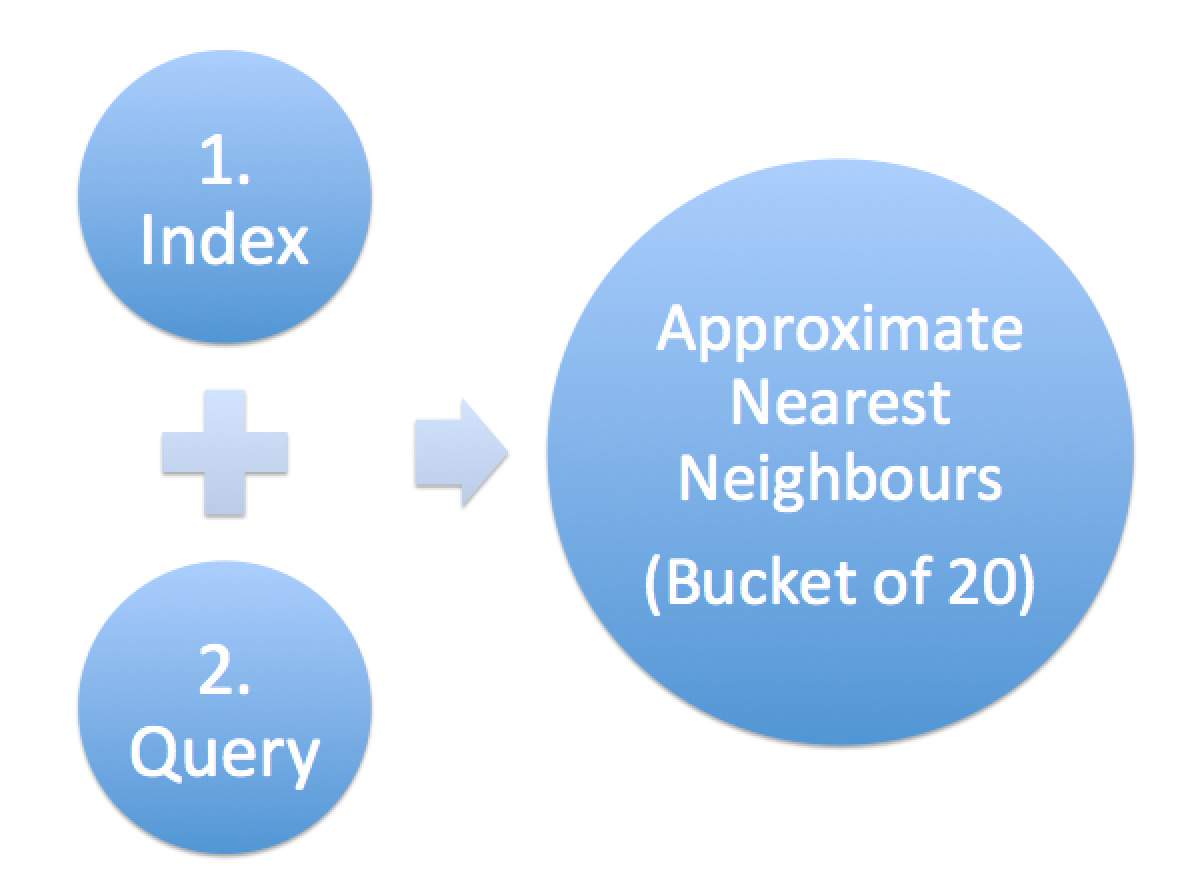
\includegraphics[width=0.35\textwidth]{./plots/ApproximateNearestNeighbours.jpeg}
\caption{There are two steps in the approximate nearest neighbour method. First create an index from the positions of all hits in the event. Then query hits to find the nearest neighbours to each hit.}
\label{fig:ApproximateNearestNeighbours}.
\end{figure}

\ \\The first step takes as input the $x$, $y$, $z$ coordinates of all the reconstructed hits in an event and returns as output a tree that groups the hits along their direction relative to the centre of the detector. The tree is built using random projections. At every node, a random sample of two hits is selected and the hyper-plane equidistant to both hits is chosen to divide the space into two further subspaces. This is done k times, to obtain an ensemble method of a forest of trees. k is a hyper-parameter to tune and is set to 10 in our study. The result is called an \emph{index}. 

\ \\In the second step, a query hit is given and the N-nearest-neighbour hits along the direction are returned (including the query hit), where N is a parameter chosen by the user. The resulting group of hits is called a \emph{bucket} or a \emph{hash} of hits. The operation is done for every hit in the event, resulting in as many buckets as there are hits in the event. The procedure is then repeated for each event in the sample.

\ \\There are several code implementations of the Approximate Nearest Neighbors algorithm. In this project the implementation in the Annoy library (Approximate Nearest Neighbors Oh Yeah)~\cite{Annoy} is used. Annoy is fast, since it is coded in C++, but easy to use from Python as the library provides a Python wrapper (or bindings). Annoy is an efficient library because a static read-only file is produced for the index, allowing it to be queried simultaneously in parallel by many threads, like when running on several CPU cores, or a GPU, or in a real production environment. The Annoy implementation supports the two step process described above: building one index made of trees and querying in parallel for several points.

\ \\Since the count of the number of hits in a truth particle tails off just before 20, as can be seen in Figure~\ref{fig:TruthParticleNbHits}, the number of hits per bucket is chosen to be 20. The pseudo-code used in this project to produce a bucket for each hit in each of the 100 events is described in Appendix~\ref{sec:AppendixPseudoCodeInputOutput}.

\section{Buckets}
\label{sec:Buckets}

With the procedure above the distribution of the size of the majority particle, defined in Section~\ref{sec:Question} and denoted \nbPositiveHit, is obtained and illustrated in Figure~\ref{fig:BucketNbPositiveHit}. This is done for both the Train and Test samples that are described later in Section~\ref{sec:TrainAndTest}. The mean and rms of the histograms are 8.5 and 2.8, respectively. The interpretation is that the average bucket contains fewer than 10 hits belonging to the same particle.  

\begin{figure}[htb]
\centering
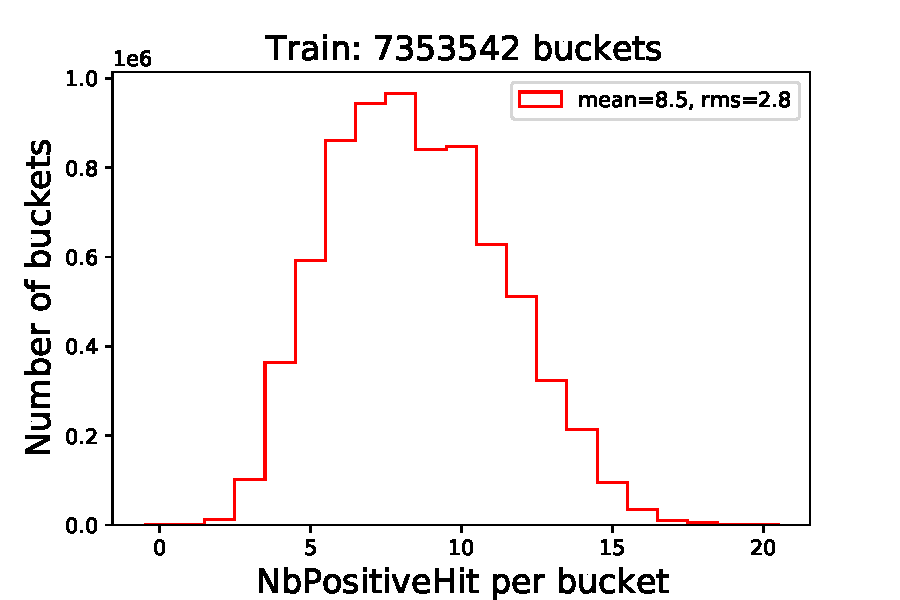
\includegraphics[width=0.34\textwidth]{plots/plot_bucket_unbalanced_Train_2.pdf}
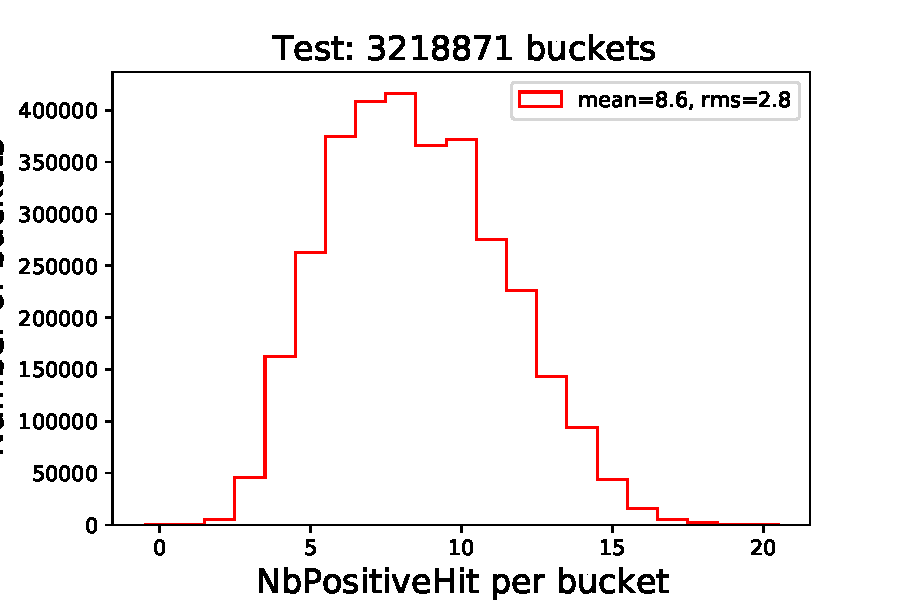
\includegraphics[width=0.34\textwidth]{plots/plot_bucket_unbalanced_Test_2.pdf}
\caption{Distribution of the majority particle size, or \nbPositiveHit}
\label{fig:BucketNbPositiveHit}.
\end{figure}

\ \\Similar to the reconstructed hits above, another aspect realised from Figure~\ref{fig:TruthParticleNbHits} is that only a fraction of truth particles have a number of hits smaller than 10. It is desired to reconstruct a particle with a significant number of hits in the bucket. A threshold of 10 is chosen. If a bucket has $\nbPositiveHit < 10$, then all its hit labels are set artificially to -1, leading to it having $\nbPositiveHit = 0$. In Figure~\ref{fig:BucketUnbalanced} the default threshold of 0 (Min00) and the chosen threshold of 10 (Min10) are overlaid for both the Train and Test samples. The Train and Test samples represent 70\% and 30\% of the events, respectively, as detailed in Section~\ref{sec:TrainAndTest}, and behave similarly. For each sample, the histograms for $\nbPositiveHit \ge 10$ are identical (visualised as one colour, blue). After this change the imbalance between the fraction of positive and negative hits is increased in the favor of the negative hits. A further balancing is needed, as described in Section~\ref{sec:BalancingDatasets}. 

\begin{figure}[htb]
\centering
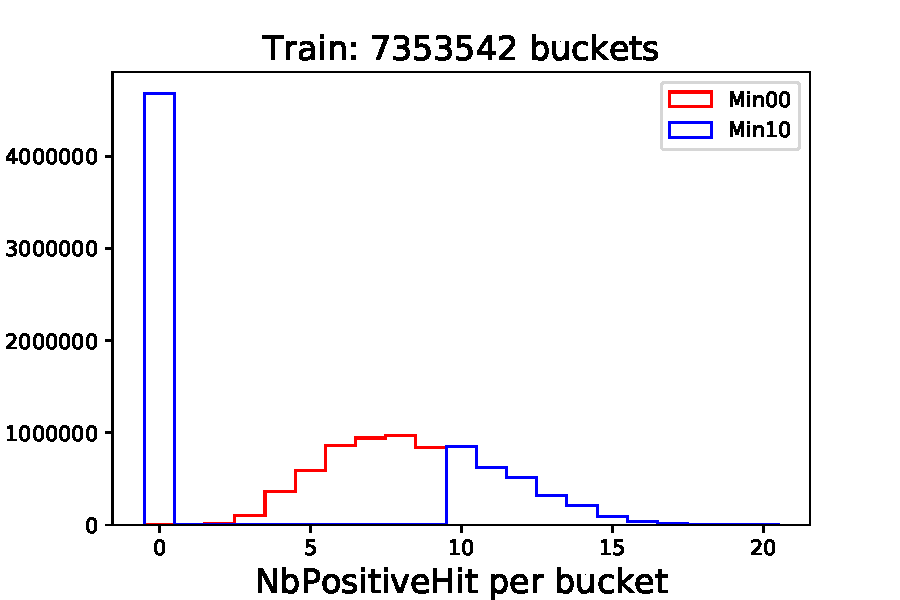
\includegraphics[width=0.34\textwidth]{plots/plot_bucket_unbalanced_Train.pdf}
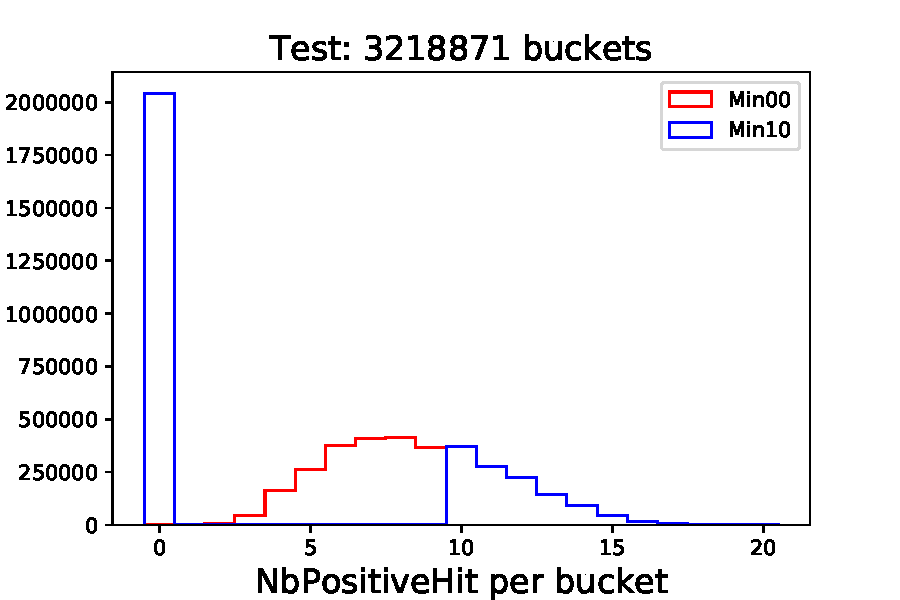
\includegraphics[width=0.34\textwidth]{plots/plot_bucket_unbalanced_Test.pdf}
\caption{Overlay of the number of positive hits per bucket by default (Min00) and after moving all hits to negative for buckets with less than 10 number of positive hits (Min10). Train (left) vs Test (right).}
\label{fig:BucketUnbalanced}
\end{figure}

\section{Multi-Label Binary Classification}
\label{sec:MultiLabelBinaryClassification}

To mathematically formulate the track reconstruction, for each bucket one must ask as many questions as there are hits in the bucket. Does the hit belong to the majority particle, equivalent to asking whether it has the label +1 (signal) or -1 (background)? For a single hit, it is a classification problem. For the entire bucket, it is a multi-label classification problem. This can be answered via a supervised machine learning model. It is a supervised problem, as the labels are known. It is a classification problem, as the answers are categorical (yes or no, +1 or -1). There are only two possible answers, so it is a binary classification. It is a multi-label classification, as for each data sample (bucket), several questions are asked (one for each hit). The exact procedure is described in detail in Chapter~\ref{chapter:MachineLearning}.
